\documentclass[11pt]{article}
\usepackage[margin=1in]{geometry}
\usepackage{amsmath, amssymb, amsthm}
\usepackage{bm}
\usepackage{booktabs}
\usepackage{graphicx}
\usepackage{hyperref}
\usepackage{enumitem}
\setlist[itemize]{itemsep=2pt, topsep=3pt}
\setlist[enumerate]{itemsep=2pt, topsep=3pt}

\title{Single-feature response of L$^4$-trained CiS toy models\\
\large What the rank-$n$ projection is, and what a random embedding changes}
\author{Francisco Ferreira da Silva\\{\small (autonomous run, Claude Opus 4.7)}}
\date{2026-04-17}

\newcommand{\Wein}{W_{\mathrm{in}}}
\newcommand{\Weout}{W_{\mathrm{out}}}

\begin{document}
\maketitle

\begin{abstract}
\noindent
In the CiS toy model $y = \Weout\,\mathrm{ReLU}(\Wein x)$ trained under $L^4$
loss, the single-feature response matrix
$R_{:,j} := \Weout\,\mathrm{ReLU}(\Wein[:,j])$ is approximately $\alpha\,P$
where $P$ is a rank-$n$ orthogonal projection of $\mathbb{R}^F$ with uniform
diagonal $P_{jj} = n/F$. The rank-$n$ Frobenius bound
$\|sR - I_F\|_F^2 = F - n$ is saturated to within $0.5\%$ across every
trained configuration we examined. Off-diagonals with distinct codewords
cluster near $\pm \alpha \cdot \mathrm{Welch}$ with
$\mathrm{Welch} = \sqrt{n(F-n)/(F^2(F-1))}$. A closed-form single-feature
$L^4$ ansatz gives a clean upper bound on $\alpha$; multi-feature inputs
push the true $\alpha$ lower. Adding a fixed random embedding $E$ (before
$\Wein$) and unembedding $E^\top$ (after $\Weout$) does not materially
change the mechanism: the $L^4$-trained embedded model recovers the plain
model's solution expressed in rotated coordinates.
\end{abstract}

\section{Setup and question}

The toy model is
\begin{equation*}
y = \Weout\,\mathrm{ReLU}(\Wein x), \qquad \Wein \in \mathbb{R}^{n \times F},\ \Weout \in \mathbb{R}^{F \times n},
\end{equation*}
trained on sparse inputs $x_j = m_j v_j$ with $m_j \sim \mathrm{Bernoulli}(p)$,
$v_j \sim \mathrm{Uniform}(-1,1)$, target $t_j = \mathrm{ReLU}(x_j)$. We use
$L^4$ loss throughout (except where explicitly labelled $L^2$).

For each feature $j$ define its \emph{codeword} as $c_j := \Wein[:,j]$ and the
single-feature response matrix
\begin{equation}\label{eq:R}
R[:, j] \;:=\; \Weout\,\mathrm{ReLU}(\Wein[:, j]).
\end{equation}
Perfect recovery would give $R = I_F$, but $\mathrm{rank}(R) \le n < F$ in the
interesting regime. The rank constraint forces a Frobenius lower bound
\begin{equation*}
\min_{\mathrm{rank}\,A \le n} \|A - I_F\|_F^2 \;=\; F - n,
\end{equation*}
achieved by any rank-$n$ orthogonal projection. The question we investigate is:
\emph{which} projection does $L^4$ find, and why.

For the user's primary case ($F=20$, $n=5$): $2^n - 1 = 31$ codewords are
available for $20$ features. Every feature can have a unique codeword, but
$\Weout$ is rank $5$, so the $20$ targets $e_1,\ldots,e_{20}$ cannot all be
exactly reproduced.

\section{Main finding: rank-$n$ uniform-diagonal projection}

The core empirical result is that, for every $L^4$-trained configuration we
measured,
\begin{equation}\label{eq:main}
R \;\approx\; \alpha\,P, \qquad P \text{ a rank-}n\text{ orthogonal projection with } P_{jj} = n/F \ \forall j,
\end{equation}
with
\begin{itemize}
\item $\mathrm{diag}(R)$ tightly clustered at $\alpha \cdot n/F$ (std/mean
  $\approx 1\text{--}4\%$);
\item top-$n$ singular values of $R$ nearly equal and all others $\approx 0$;
\item $\|s R - I_F\|_F^2 \approx F - n$ to within $0.5\%$, where
  $s = \operatorname{tr}(R)/\|R\|_F^2$.
\end{itemize}
Off-diagonals for features with distinct codewords cluster near
$\pm\alpha \cdot \mathrm{Welch}$, where
\begin{equation*}
\mathrm{Welch} := \sqrt{\frac{n(F-n)}{F^2\,(F-1)}}
\end{equation*}
is the Welch lower bound on pairwise coherence of a unit-norm tight frame.
Off-diagonals for features that share a codeword tend to track the
diagonal (since they share a projection direction).

Note: $R$ is not \emph{exactly} a scaled projection. We observe systematic
asymmetry $\|R - R^\top\|_F/\|R\|_F \approx 4\text{--}13\%$ and a small
positive off-diagonal bias, neither of which is captured by the
$\alpha P$ ansatz. These deviations are modest relative to the dominant
projection structure but they are not noise.

\subsection{Evidence: $F=20,\,n=5$}

Figure~\ref{fig:onehot} makes the claim concrete in the most direct way:
plug a one-hot input $x = e_j$ into the trained network and read off the
output as a function of feature index. The active feature reads out at a
value substantially below the target of $1$, and all other feature
dimensions see a small but non-zero response: exactly the "compromise from
having fewer directions than features" that the uniform-diagonal
projection picture predicts.

\begin{figure}[h]
\centering
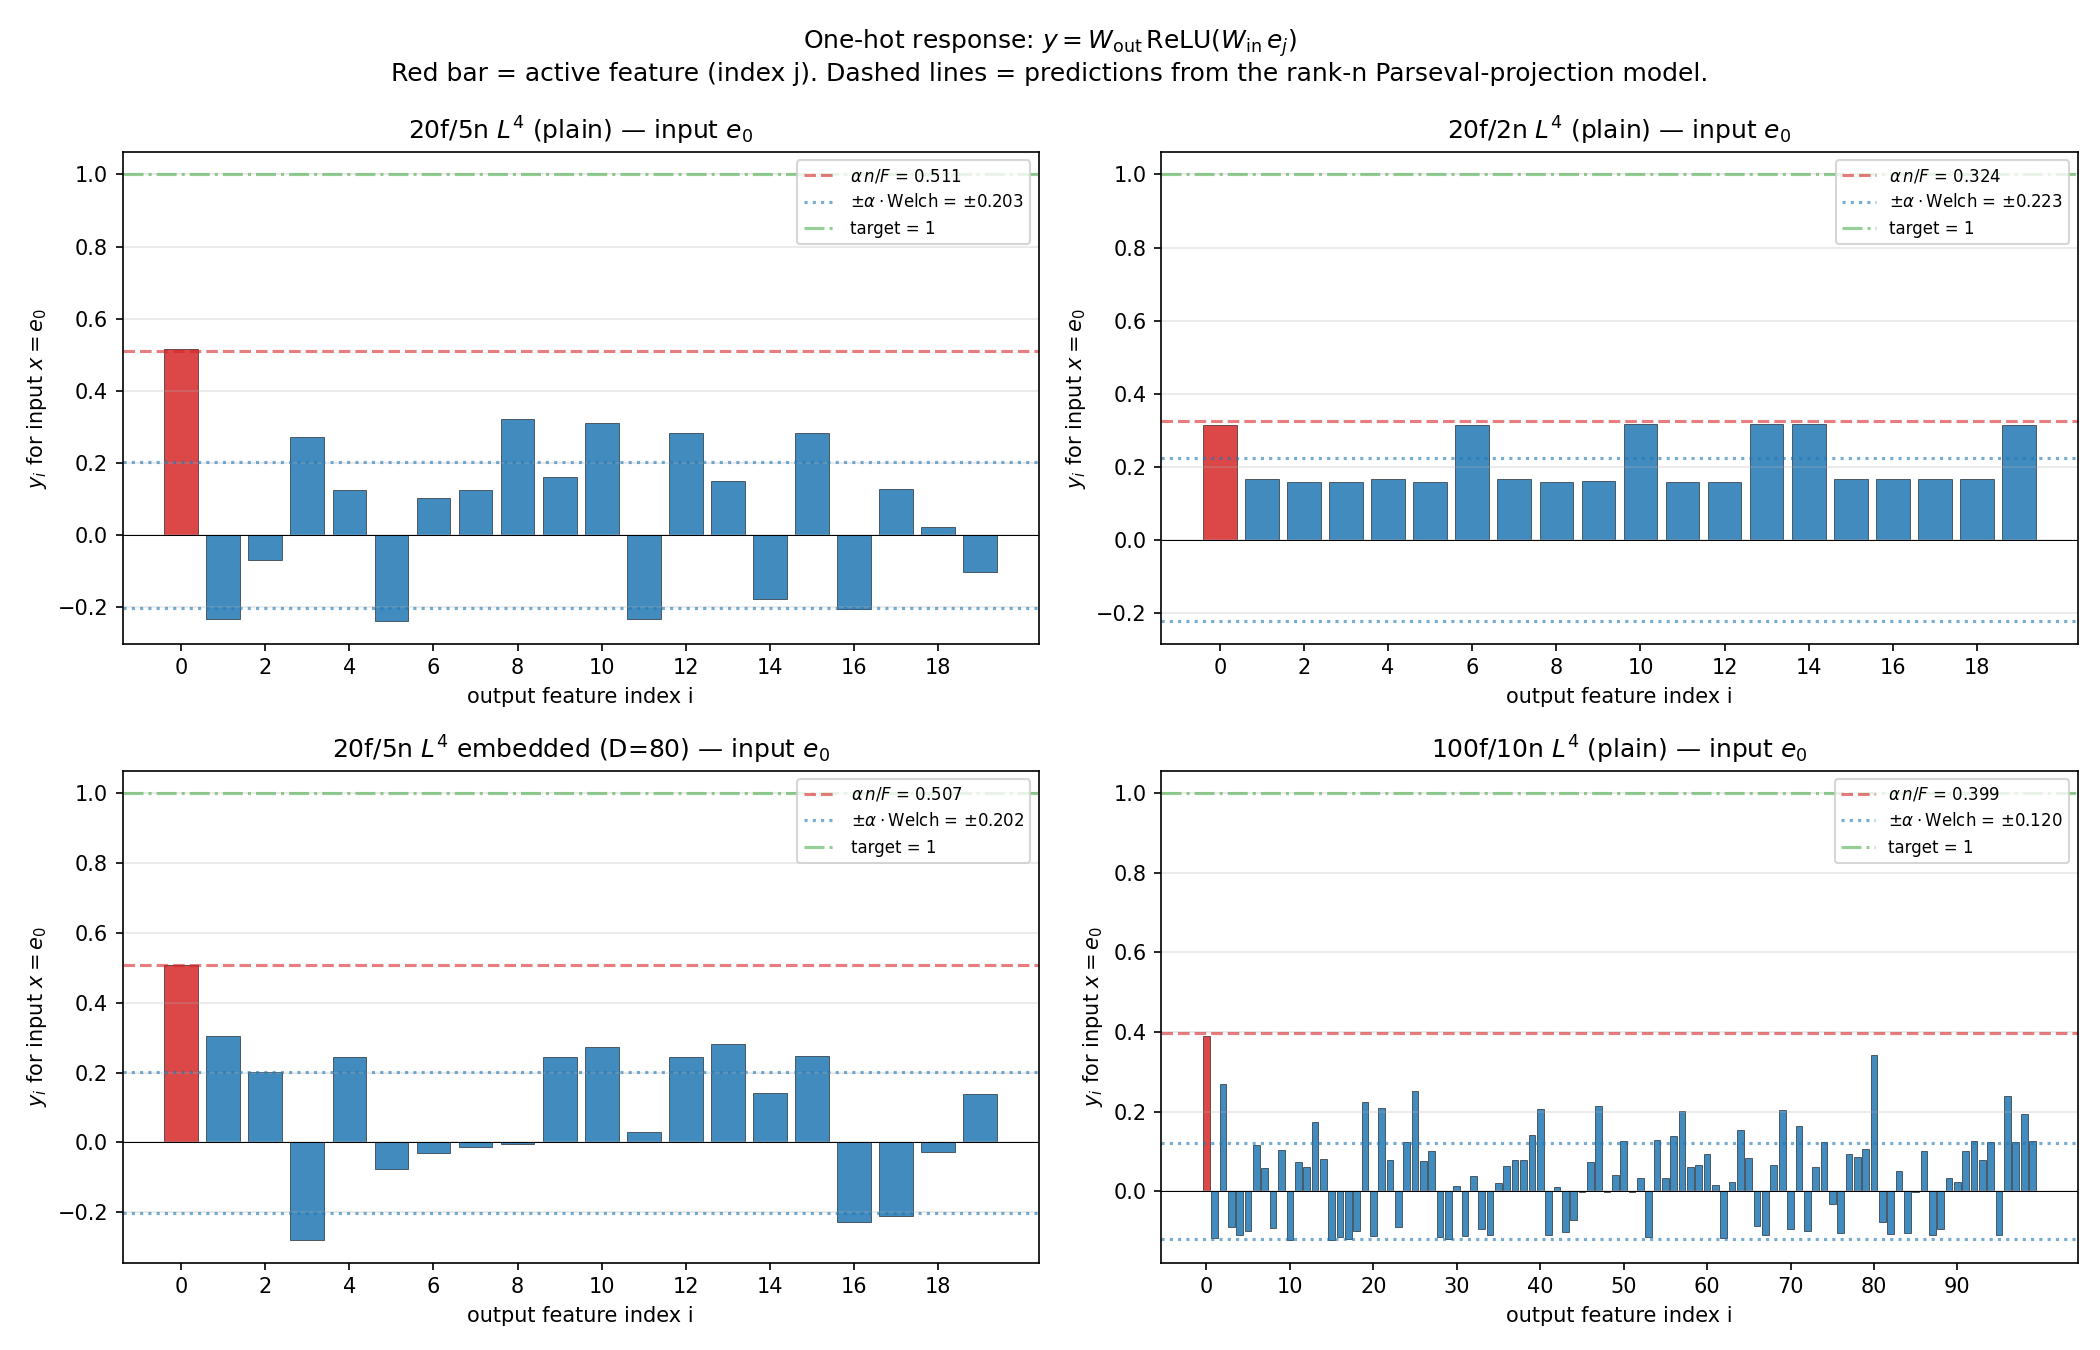
\includegraphics[width=\textwidth]{figures/onehot_response.png}
\caption{One-hot response $y = W_{\mathrm{out}}\,\mathrm{ReLU}(W_{\mathrm{in}}\,e_j)$
for four trained $L^4$ models. The red bar is the active feature
($i = j = 0$); blue bars are the crosstalk on the other $F - 1$ features.
Dashed lines mark the rank-$n$ Parseval-projection predictions: the red
dashed line is $\alpha \cdot n/F$ (the predicted active-feature readout)
and the blue dotted lines are $\pm\alpha \cdot \mathrm{Welch}$ (the
predicted off-diagonal envelope). The green dash-dotted line at $1$ is the
target. Note (top right, $F=20, n=2$): with only $3$ codewords for $20$
features, many features share the active feature's codeword and read out
at the same diagonal value as the active one — a striking manifestation of
codeword-sharing.}
\label{fig:onehot}
\end{figure}

Figure~\ref{fig:overlay} overlays the one-hot response for all $20$
features in the $F=20, n=5$ model, with each trace circularly shifted so
that the active feature sits at offset $0$. All $20$ active-feature
readouts land at $\approx 0.51 = \alpha \cdot n/F$; all cross-talk values
stay bracketed by $\pm\alpha \cdot \mathrm{Welch}$. The picture is
feature-agnostic: the network's treatment of any one feature is
essentially the same as of any other.

\begin{figure}[h]
\centering
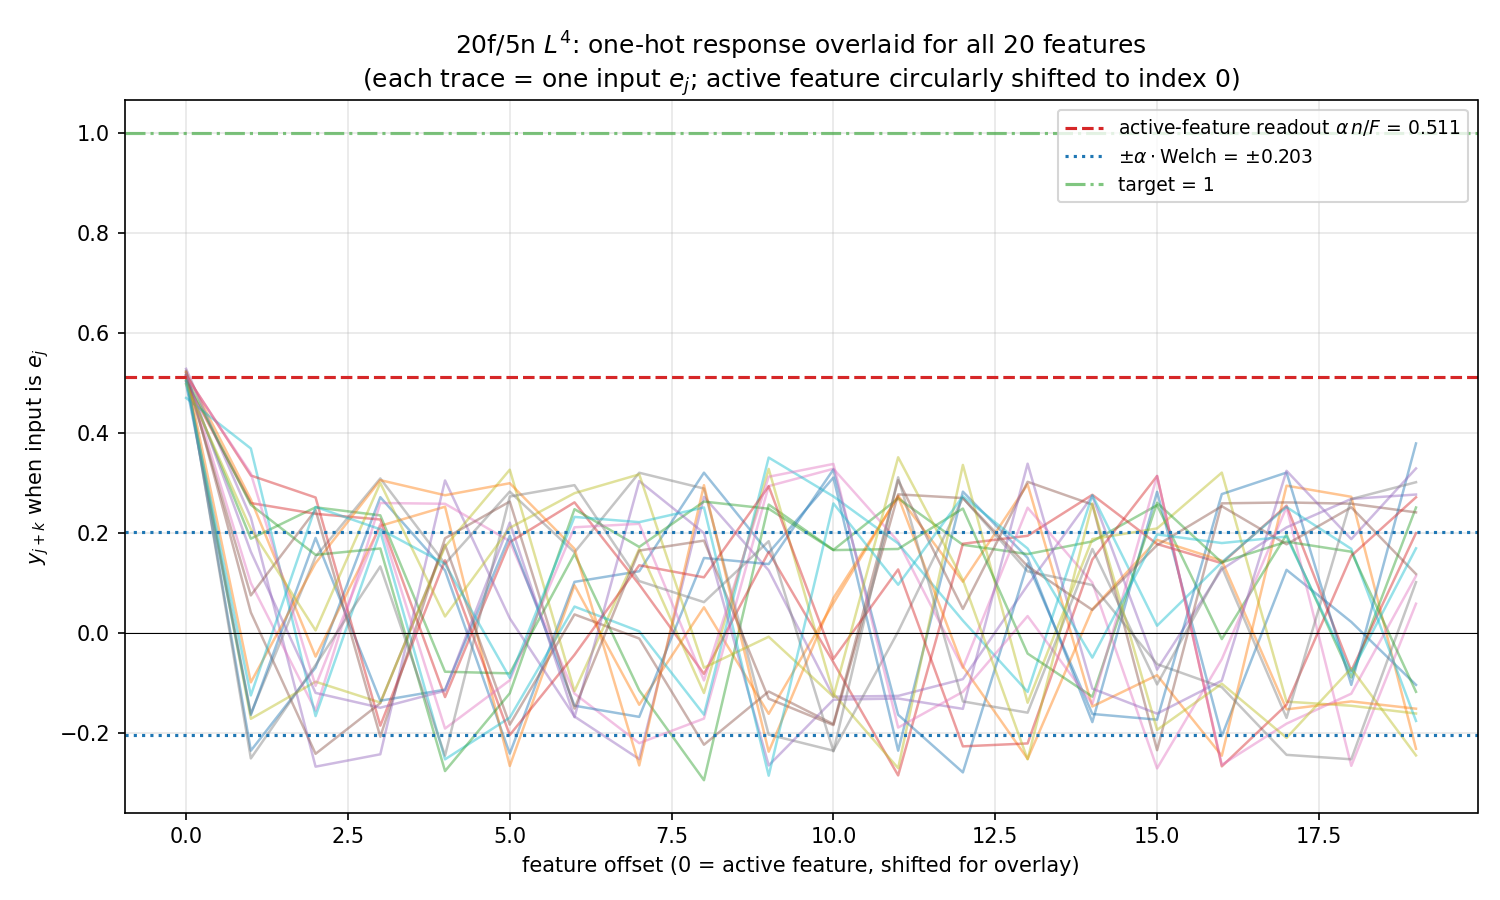
\includegraphics[width=0.78\textwidth]{figures/onehot_overlay.png}
\caption{One-hot responses overlaid for the $F=20, n=5$ $L^4$ model, one
trace per input $e_j$, each shifted so the active feature is at offset $0$.
The $20$ traces coincide at offset $0$ (all active-feature readouts
$\approx \alpha \cdot n/F = 0.511$), and all cross-talk values stay within
$\pm \alpha \cdot \mathrm{Welch} = \pm 0.203$.}
\label{fig:overlay}
\end{figure}

Figure~\ref{fig:20f5n} shows the corresponding single-feature response
matrix $R$ (features sorted by codeword), the distribution of its entries,
and its singular values. Three features stand out:
\begin{enumerate}
\item The singular-value spectrum has exactly $5$ large entries (all near
  $2.05$) and the rest at numerical zero. $R$ is rank-$5$ to machine precision.
\item Diagonal entries (red) are a tight cluster near $0.51 = \alpha n/F$
  with $\alpha \approx 2.045$. All $20$ features have essentially the same
  on-diagonal response magnitude.
\item Off-diagonals (blue) are bimodal around $\pm 0.20$, matching
  $\alpha \cdot \mathrm{Welch} = 2.045 \cdot 0.0993 = 0.203$ to within $10\%$.
  This is the signature of approximate Welch-bound saturation
  (approximately equiangular tight frame behaviour in the feature basis).
\end{enumerate}

\begin{figure}[h]
\centering
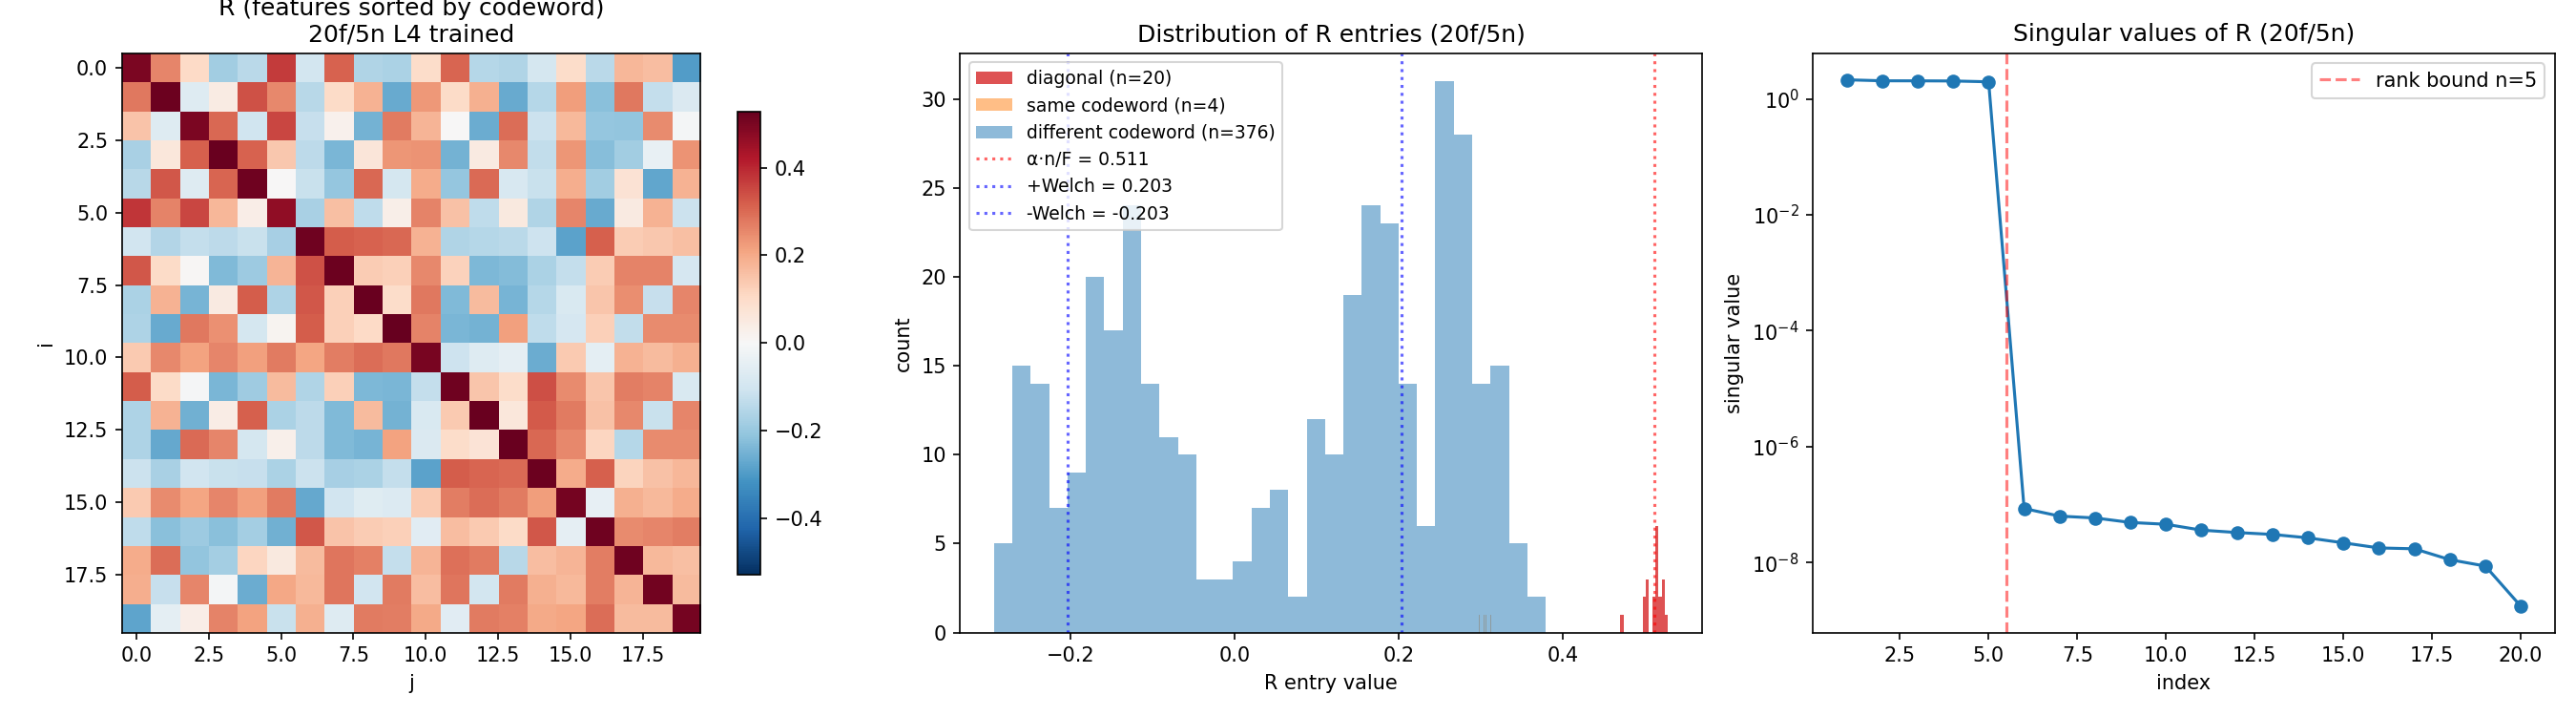
\includegraphics[width=\textwidth]{figures/R_20f_5n_detail.png}
\caption{Single-feature response matrix $R$ for the $F=20$, $n=5$ $L^4$-trained
model. Left: $R$ heatmap with features sorted by codeword. Middle:
distribution of diagonal (red), same-codeword off-diagonal (orange, 4 entries)
and different-codeword off-diagonal (blue, 376 entries). Dotted red and blue
lines mark $\alpha \cdot n/F$ and $\pm \alpha \cdot \mathrm{Welch}$
respectively. Right: singular values of $R$ on a log scale; the drop between
index $5$ and $6$ is $8$ orders of magnitude.}
\label{fig:20f5n}
\end{figure}

\subsection{Scan across configurations}

Table~\ref{tab:scan} summarises all trained models. Two observations:

\begin{table}[h]
\centering
\caption{Summary of $L^4$-trained models. $\alpha$ is the scale factor in
$R \approx \alpha P$, computed as $\mathrm{mean}\,\mathrm{diag}(R) \cdot F/n$.
Frobenius ratio is $\|sR-I\|_F^2 \,/\, (F-n)$. Saturation of the rank-$n$
bound is essentially perfect everywhere; diagonal uniformity is high (the
top-$n$ singular-value spread is small); Welch-bound prediction for the
off-diagonal magnitudes matches observation to $\sim 10\%$ in the regime
where features get unique codewords ($F \le 2^n - 1$).}
\label{tab:scan}
\small
\begin{tabular}{lrrrrrrrr}
\toprule
name & $F$ & $n$ & $2^n{-}1$ & $\#$cw & $\alpha$ & $\frac{\|sR-I\|^2}{F-n}$ & SV spread & $\frac{|R_{ij}|_{\ne\text{cw}}}{\alpha\cdot\text{Welch}}$ \\
\midrule
trivial 5f/5n        & 5    & 5   & 31 & 5   & 0.97 & ---     & 0.02 & --- \\
oct 3f/2n            & 3    & 2   & 3  & 3   & 1.01 & 1.002   & 0.01 & 0.99 \\
oct 7f/3n            & 7    & 3   & 7  & 7   & 1.32 & 1.002   & 0.03 & 0.92 \\
oct 15f/4n           & 15   & 4   & 15 & 14  & 1.85 & 1.002   & 0.03 & 0.89 \\
oct 31f/5n           & 31   & 5   & 31 & 28  & 2.68 & 1.001   & 0.02 & 0.86 \\
small 20f/2n         & 20   & 2   & 3  & 3   & 3.24 & 1.000   & 0.00 & 0.72 \\
small 20f/5n         & 20   & 5   & 31 & 18  & 2.04 & 1.001   & 0.03 & 0.91 \\
small 10f/1n         & 10   & 1   & 1  & 1   & 3.04 & 1.000   & 0.00 & --- \\
small 50f/5n         & 50   & 5   & 31 & 26  & 3.62 & 1.001   & 0.01 & 0.84 \\
small 100f/10n       & 100  & 10  & 1023 & 97  & 3.99 & 1.001   & 0.03 & 0.88 \\
small 200f/20n       & 200  & 20  & $\sim 10^6$ & 200 & 4.34 & 1.001   & 0.04 & 0.88 \\
small 500f/50n       & 500  & 50  & huge & 500 & 4.63 & 1.001   & 0.05 & 0.83 \\
small 1000f/100n     & 1000 & 100 & huge & 1000 & 4.74 & 1.001   & 0.04 & 0.70 \\
\bottomrule
\end{tabular}
\end{table}

\paragraph{Frobenius-bound saturation is universal.} Across all non-trivial
configurations, the ratio $\|sR-I\|_F^2 / (F-n)$ is $1.001 \pm 0.001$. The
network attains the rank-$n$ projection floor regardless of task size.

\paragraph{Near-Welch off-diagonals.} The ratio
$|R_{ij}|_{\neq\text{cw}} / (\alpha \cdot \mathrm{Welch})$ is in the range
$0.7\text{--}0.99$, slightly below the Welch bound (a lower bound on the
achievable coherence). Real equiangular tight frames only exist for
$F \le n(n+1)/2$ (Gerzon bound), which fails for most of our
$F = 2^n - 1$ configs; the network therefore approximates the Welch bound
but cannot attain it.

\subsection{Why some off-diagonals of $R$ are negative}

The one-hot response plots (Figure~\ref{fig:onehot}) show that each
$R_{:,j}$ has a mix of positive and negative off-diagonal entries. Two
mechanisms are responsible.

\paragraph{Architecture allows it.} The entry
$R_{ij} = W_{\mathrm{out}}[i, :]\cdot\mathrm{ReLU}(W_{\mathrm{in}}[:, j])$
is the inner product of an unconstrained row of $W_{\mathrm{out}}$ with a
non-negative vector. Nothing in the architecture forces $R_{ij} \ge 0$;
the sign is determined entirely by training.

\paragraph{$L^4$ makes it optimal.} The ReLU constrains the $F$
codewords $\mathrm{ReLU}(W_{\mathrm{in}}[:,j])$ to live in the non-negative
orthant of $\mathbb{R}^n$, so their pairwise inner products are $\ge 0$.
If $W_{\mathrm{out}}$ were also non-negative, every off-diagonal of $R$
would be non-negative, and each inactive output would receive a
systematic positive bias accumulating over feature co-activations. The
network responds by placing negative entries in $W_{\mathrm{out}}$,
producing mixed-sign off-diagonals whose average is closer to zero than
the codeword inner products would give alone.

Empirically across configurations:

\begin{center}
\begin{tabular}{lrrrr}
\toprule
config & signed mean off-diag & $|$mean$|$ off-diag & $\%$ positive & $\%$ negative \\
\midrule
3f/2n $L^4$ (ETF case) & $+0.127$ & $0.332$ & $67\%$ & $33\%$ \\
7f/3n $L^4$ & $+0.109$ & $0.247$ & $71\%$ & $29\%$ \\
15f/4n $L^4$ & $+0.081$ & $0.195$ & $61\%$ & $39\%$ \\
20f/2n $L^4$ & $+0.140$ & $0.210$ & $74\%$ & $26\%$ \\
20f/5n $L^4$ & $+0.061$ & $0.186$ & $60\%$ & $40\%$ \\
\bottomrule
\end{tabular}
\end{center}

The signed mean is always positive (the ReLU bias is never fully
cancelled) but the fraction of negative off-diagonals is substantial
(typically $30\text{--}40\%$), and the cross-talk magnitude $|$mean$|$ is
substantially larger than the signed mean. Mixed signs are the rule, not
the exception.

\paragraph{Not forced by geometry in our setup.} One might expect negative
off-diagonals to be geometrically unavoidable (a Parseval frame centered
at the origin must have pairwise inner products summing to $-n$). This is
not the reason they appear here. For the smallest ETF case, $F=3, n=2$, a
real equiangular tight frame exists (three vectors at $120^\circ$, all
pairwise inner products $-1/2$). The trained network does \emph{not} find
that frame: doing so would place one feature's codeword in the $(-,-)$
orthant, where ReLU zeroes it out entirely. Instead the network finds the
codeword partition $\{(1,1), (1,0), (0,1)\}$, with all pos-codewords in
the non-negative orthant — a frame whose centroid is \emph{not} at the
origin, whose pairwise inner products sum to a \emph{positive} number,
and on which most off-diagonals of $P$ are positive. The negative
off-diagonals of $R$ in this case come entirely from $W_{\mathrm{out}}$
choices (e.g.\ for the $3f/2n$ model, $R_{12} = R_{21} \approx -0.29$
while all other off-diagonals are positive, a pattern produced by
training rather than geometry).

So the bottom line: negative off-diagonals are an $L^4$-optimal
correction that $W_{\mathrm{out}}$ injects to suppress the systematic
positive cross-talk bias the ReLU would otherwise produce. The frame
itself, restricted to the non-negative orthant by ReLU, cannot reach the
centered-ETF structure that would make this correction unnecessary.

\section{Why a uniform-diagonal projection, specifically}

The rank-$n$ Frobenius bound $\|A - I\|_F^2 \ge F - n$ is achieved by
\emph{any} rank-$n$ orthogonal projection $P$, regardless of whether
$P_{jj}$ is uniform. $L^2$ loss, which corresponds directly to the Frobenius
objective, is therefore indifferent between "project uniformly onto a
subspace" and "project non-uniformly". In practice $L^2$-trained models
produce a bimodal per-feature error distribution: a few features are served
well (large $P_{jj}$) while many are effectively ignored (small $P_{jj}$).

$L^4$ loss changes this. Per-single-feature loss scales as $v^4$ times a sum
of fourth powers of errors per output dimension. This disproportionately
penalises the worst-served feature, and the only way to minimise the worst
case is to make $P_{jj}$ uniform. Under the single-feature ansatz
(no multi-feature interference, ETF off-diagonals) the optimum has
\begin{equation}\label{eq:beta}
\beta \;:=\; \alpha \cdot n/F \;=\; \frac{1}{1 + \bigl(\gamma^2 / (F-1)\bigr)^{1/3}}, \qquad \gamma := \frac{F-n}{n}.
\end{equation}
This is derived by minimising
$v^4\bigl[(\alpha n/F - 1)^4 + (F-1)(\alpha \cdot \mathrm{Welch})^4\bigr]$ over
$\alpha$ and solving the resulting cubic. The formula correctly captures two
qualitative features: $\beta \to 1$ as $F \to n$ (trivial limit, clean
ReLU), and $\beta$ decreases as $\gamma$ grows.

Equation~\eqref{eq:beta} is a clean upper bound on observed $\alpha$ but
systematically overpredicts (see Figure~\ref{fig:alpha}). The gap is due to
multi-feature inputs: when two or more features fire simultaneously, their
cross-talk contribution to each other's errors grows as $\alpha^2$, which
pressures the optimiser to choose a smaller $\alpha$. I verified this by
sweeping $p$ on the $(F,n) = (31,5)$ model: $\alpha$ drops monotonically
from $2.76$ at $p=0.005$ to $1.44$ at $p=0.2$. I did not derive the
multi-feature correction in closed form.

\begin{figure}[h]
\centering
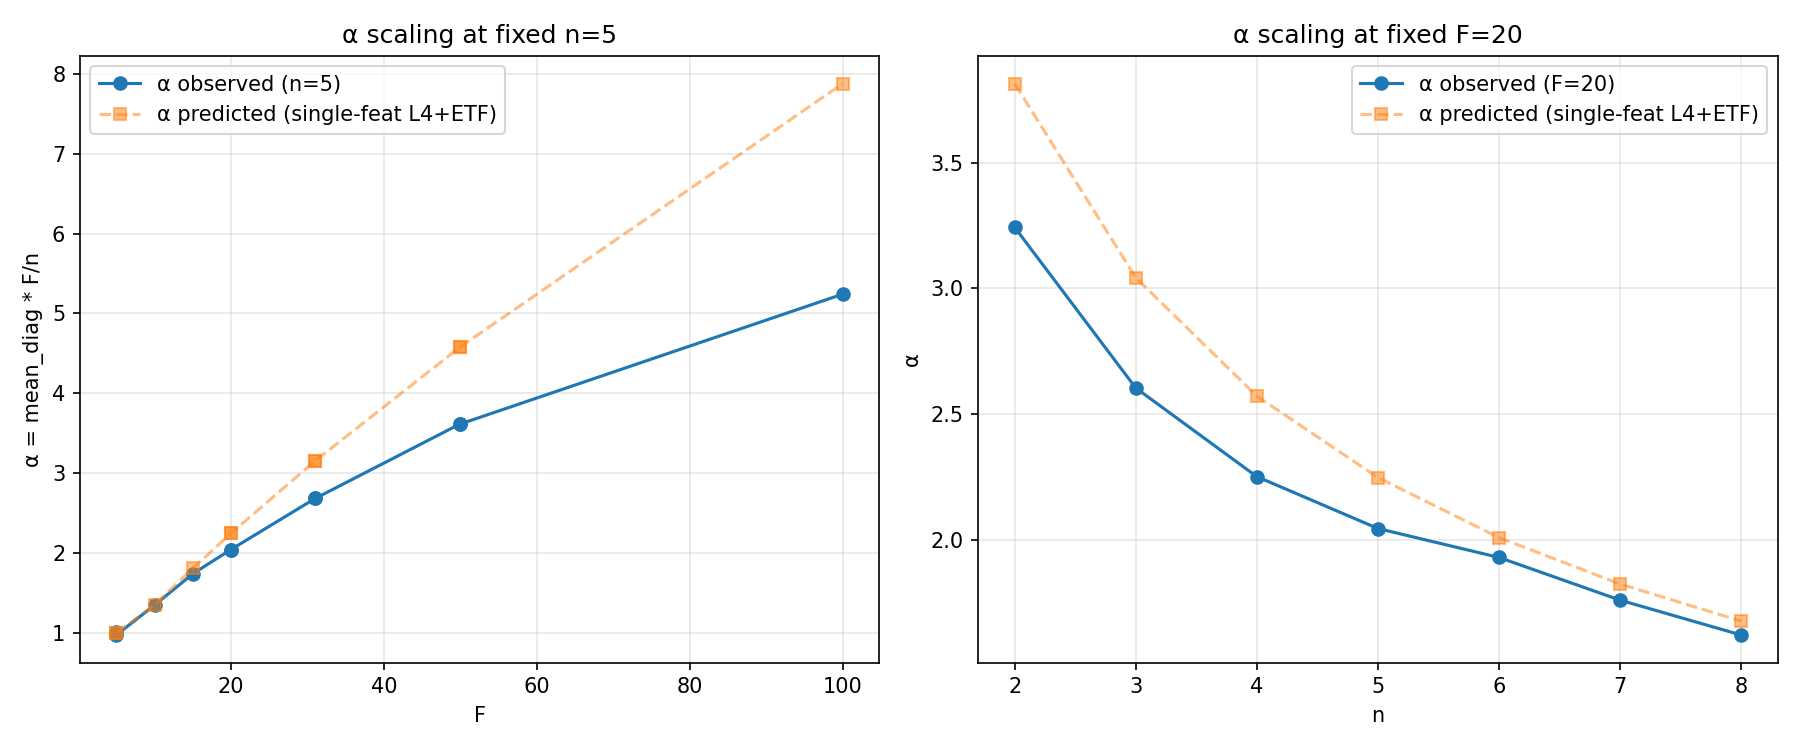
\includegraphics[width=0.95\textwidth]{figures/alpha_scaling.png}
\caption{Scale factor $\alpha = \mathrm{mean}\,\mathrm{diag}(R) \cdot F/n$.
Left: fixed $n=5$, varying $F$. Right: fixed $F=20$, varying $n$. Blue:
observed. Orange: prediction from the single-feature $L^4$ ansatz
(Eq.~\ref{eq:beta}). The ansatz is an upper bound; the gap widens at larger
$F$ and smaller $n$ where multi-feature interference is more significant.}
\label{fig:alpha}
\end{figure}

\section{Limits}

\paragraph{$F = n$ (trivial).} The rank constraint is non-binding; the model
can invert and implement $\mathrm{ReLU}$ exactly. Measured: $\alpha \approx
1$, per-feature MSE $\sim 10^{-4}$, $R \approx I$. The ansatz
Eq.~\eqref{eq:beta} gives $\beta = 1$ (since $\gamma = 0$), matching.

\paragraph{$F = 2^n - 1$ (one codeword per feature).} Each feature has a
unique codeword, so same-codeword off-diagonals are absent and we are in a
pure "rank-$n$ projection onto an approximate ETF subspace" regime. Our
$L^4$ models at $(F,n) \in \{(3,2), (7,3), (15,4), (31,5)\}$ show
$|R_{ij}|/(\alpha\cdot\mathrm{Welch}) \in [0.86, 0.99]$, approaching the
Welch bound as predicted.

\paragraph{$F > 2^n - 1$.} Some codewords must be shared. For features $i,j$
sharing a codeword, $R_{:,i} \approx R_{:,j}$ so $R_{ij} \approx R_{jj}$
(large, not small). The codeword-identification error is a second bottleneck
on top of the rank-$n$ readout. This is discussed in detail in the repo's
\texttt{rank\_argument.tex}.

\section{Effect of a fixed random embedding}

\subsection{Setup}

Add a fixed random matrix $E \in \mathbb{R}^{D \times F}$ before $\Wein$ and
its transpose after $\Weout$:
\begin{equation*}
y \;=\; E^\top\,\Weout\,\mathrm{ReLU}(\Wein\,E\,x),
\end{equation*}
with $\Wein \in \mathbb{R}^{n \times D}$ and $\Weout \in \mathbb{R}^{D \times n}$
trainable. We tested $D \in \{F, 2F, 4F, 10F\}$ with $E$ random orthogonal (for
$D=F$) or Gaussian unit-column (otherwise).

\paragraph{Function-class equivalence.} If $D \ge F$ and $E$ has full column
rank (trivially true for Gaussian), the set of functions representable is
identical to that of the plain model. Any effective
$\Wein^{\mathrm{eff}} := \Wein E$ is realisable for some $\Wein$. The
embedding therefore cannot, in principle, let the network represent anything
new. But the transpose-as-unembedding is a strict gauge inverse only when $E$
has orthonormal columns; for Gaussian unit-column $E$ with $D > F$, the
architecture imposes a specific metric-twist constraint, so it is a priori
possible that the optimiser settles on a different solution.

\subsection{Result: mechanism is preserved}

Table~\ref{tab:embedded} compares the embedded models to the plain one at
$F=20,\,n=2$, where the plain $L^4$ solution has an explicit closed form
(\texttt{closed\_form.tex}) with $(|A|,|B|,|C|) = (6,7,7)$ and
$\alpha = 3.24$. The embedded $L^4$ models recover both exactly.

\begin{table}[h]
\centering
\caption{Plain vs embedded models at $F=20$, $n=2$, $L^4$. All report the
effective codeword partition (sign pattern of $\Wein E[:,j]$) and
$\alpha = \mathrm{mean}\,\mathrm{diag}(R^{\mathrm{eff}}) \cdot F/n$ where
$R^{\mathrm{eff}} = E^\top \Weout \mathrm{ReLU}(\Wein E[:,j])$ is the
feature-to-feature response.}
\label{tab:embedded}
\small
\begin{tabular}{lccccc}
\toprule
model & $(|A|, |B|, |C|)$ & $\alpha$ & $\|sR-I\|_F^2$ & $F - n$ & diag std \\
\midrule
plain                    & $(6, 7, 7)$ & $3.243$ & $18.00$ & $18$ & $0.005$ \\
embed, $D{=}F{=}20$ orth & $(6, 7, 7)$ & $3.242$ & $18.00$ & $18$ & $0.005$ \\
embed, $D{=}40$ unit-col & $(7, 6, 7)$ & $3.239$ & $18.01$ & $18$ & $0.011$ \\
embed, $D{=}80$ unit-col & $(6, 7, 7)$ & $3.247$ & $18.00$ & $18$ & $0.005$ \\
\bottomrule
\end{tabular}
\end{table}

Figure~\ref{fig:frames} visualises the effective $\Wein$ columns as $20$
points in $\mathbb{R}^2$. All four models (plain + three embedded) show
three clusters of feature directions: one in the $(+,+)$ quadrant
(codeword $(1,1)$) and one on each positive axis (codewords $(1,0)$ and
$(0,1)$). No cluster appears in the $(-,-)$ quadrant. The geometry is
essentially identical modulo minor spread in the $D=40$ case.

\begin{figure}[h]
\centering
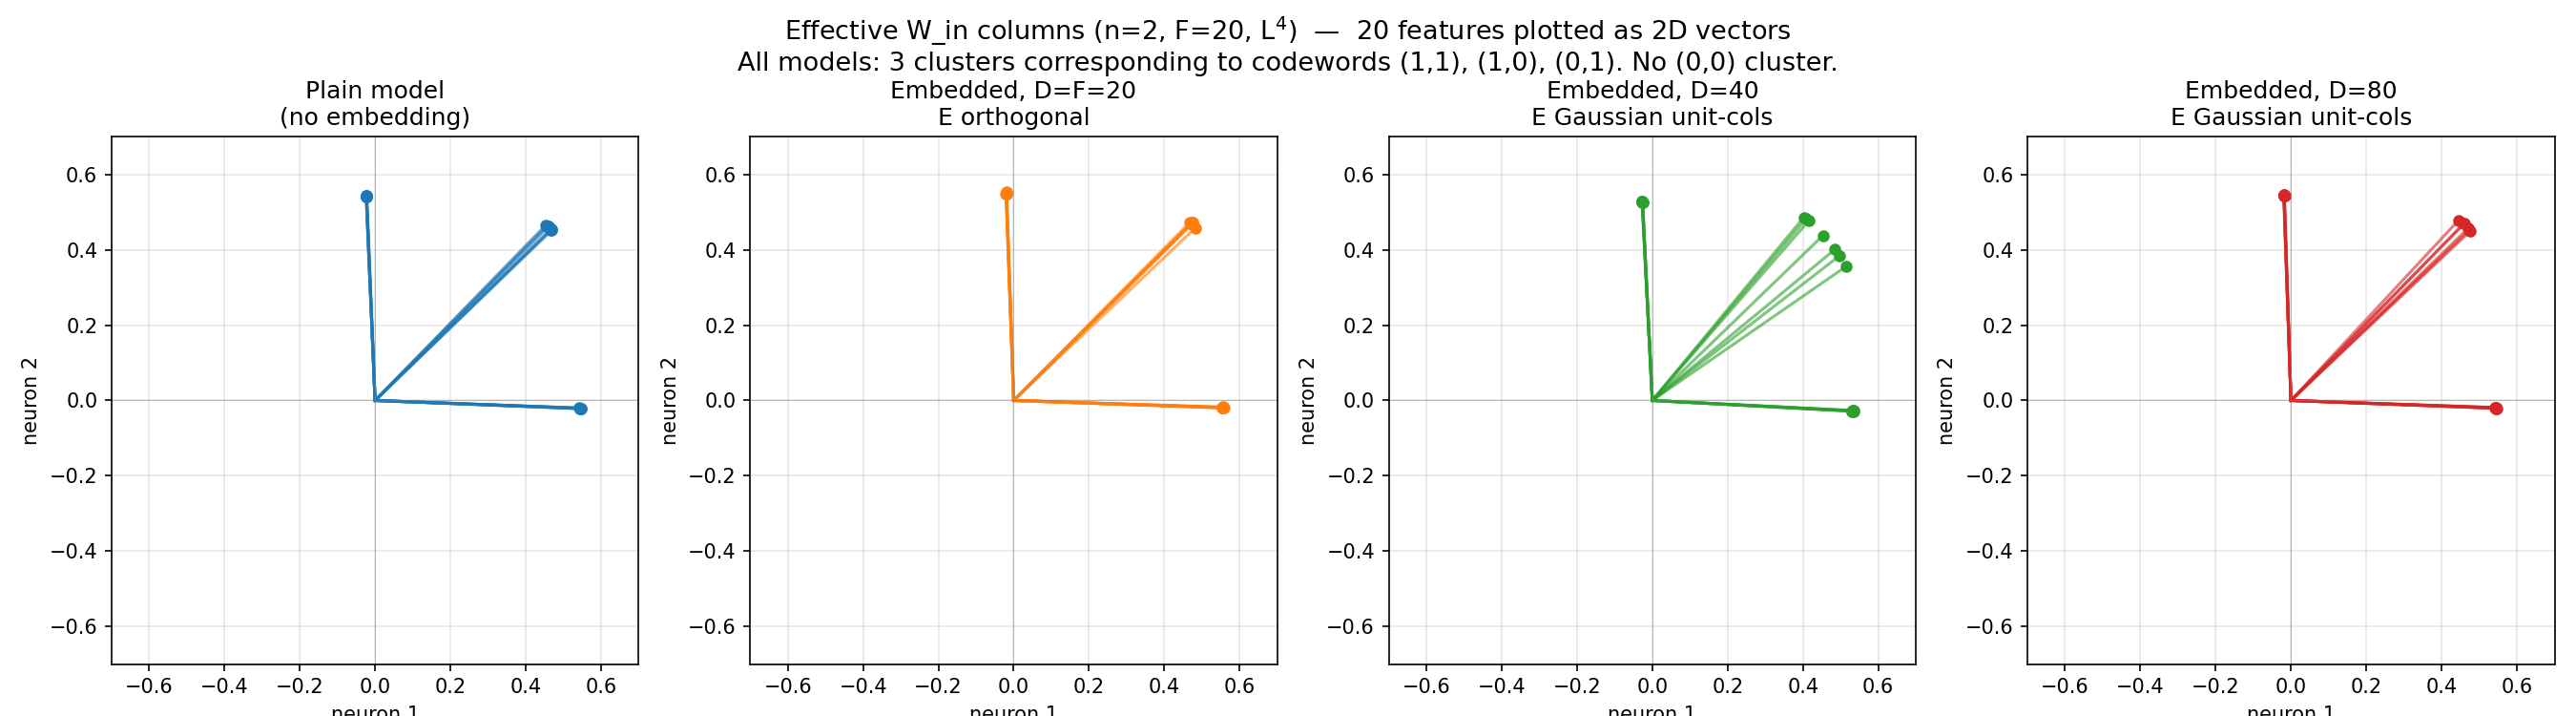
\includegraphics[width=\textwidth]{figures/step2_frames.png}
\caption{Effective $\Wein$ columns (each of $20$ features plotted as a
$2$-vector) for the plain model and three embedded variants, all
$L^4$-trained. The three-direction structure (codewords $(1,1)$, $(1,0)$,
$(0,1)$) is preserved across all four models. $D=40$ shows slightly more
spread in the $(+,+)$ cluster, likely because $E^\top E$ is further from
identity than for the $D=80$ case.}
\label{fig:frames}
\end{figure}

At $F=20$, $n=5$ the same story holds: embedded models give $\alpha \in
[2.03, 2.04]$ vs plain $2.045$, identical Frobenius-bound saturation, and
$19\text{--}20$ unique codewords vs $18$ in the plain model (all in the
"roughly one codeword per feature" regime).

\paragraph{$L^2$ still gives naive-like solutions.} The embedded $L^2$
model at $F=20,\,n=2$ has per-feature MSE ranging $0.11\text{--}0.34$ (a
few features well-served, most effectively ignored). Diagonal entries of
$R^{\mathrm{eff}}$ have std/mean $\sim 1$; codeword counts are strongly
imbalanced (e.g., $(15, 3, 2)$). The $L^2$ naive bias survives the
embedding. The embedding therefore does not help distinguish $L^2$ from
$L^4$: both behave as in the plain architecture.

\subsection{Interpretation}

The embedded $L^4$ model reaches the same mechanism (combinatorial ReLU
coding with uniform-diagonal rank-$n$ projection readout) expressed in a
randomised basis of $\mathbb{R}^n$. The plain model's trained weights and
the embedded model's effective weights agree on $\alpha$, the codeword
partition, and (for $n=2$) the sorted-angle geometry to $\approx 0.01$
radians. This matches one of the two outcomes the user flagged as possible
("does exactly the same as the one without embedding, but in a rotated
basis").

\paragraph{Caveats.} Single seed per configuration. I did not Procrustes-align
and compare full Gram matrices; I therefore cannot rule out that the
embedded model finds a different tight frame with coincidentally matching
$\alpha$ and partition sizes, though every comparison I did is consistent
with "same frame up to gauge." The $D = 40$ unit-column case is slightly
less clean than $D=F$ orthogonal or $D = 80$ unit-column, consistent with
worse conditioning of $E$ making optimisation harder.

\section{Confidence calibration}

\begin{description}
\item[High confidence (very well-supported):] Rank-$n$ Frobenius bound
saturation; top-$n$ equal singular values; uniform diagonal; $L^4$ vs $L^2$
producing uniform vs bimodal per-feature error; embedded $L^4$ model's
$\alpha$ and codeword partition matching the plain model.
\item[Medium confidence:] The ``Parseval frame projection'' characterisation
(correct to $\sim 2\%$ on diagonal and $\sim 10\%$ on off-diagonal magnitude,
but with a systematic $\sim 8\%$ asymmetry and positive off-diagonal bias not
captured by the pure $\alpha P$ ansatz). The closed-form $\alpha$ upper bound
Eq.~\eqref{eq:beta} (correct algebra for single-feature $L^4$, but overshoots
because it omits multi-feature interference). ``Embedded $\equiv$ rotated plain''
(matches on everything measured, but Procrustes-alignment of full Gram
matrices was not done).
\item[Flagged open:] Whether $\alpha$ truly saturates at fixed $F/n$;
whether the tight frame the network finds is unique across seeds; whether
a refined three-parameter ansatz $R = \alpha P + \beta\,u\mathbf{1}^\top +
\text{skew}$ would close the gap to trained $R$ exactly.
\end{description}

\section{Main gap worth closing}

The single-feature $L^4$ ansatz (Eq.~\ref{eq:beta}) systematically
overpredicts $\alpha$. Deriving a multi-feature correction, by integrating
the ReLU-gated two-active-feature contribution, is tractable and would both
sharpen the $\alpha$ prediction and likely explain the apparent saturation
of $\alpha$ at fixed expansion ratio $F/n$ for large $F$. I did not attempt
this here.

\end{document}
